\section{Existing System: \idx{ScaleNet}} % (fold)
\label{sec:scalenet}

\idx{ScaleNet} \cite{SIE06} is a research project developed between 2005 and 2009.
Partly sponsored by the \emph{German Ministry of Education}, several major corporations participated, including \emph{Deutsche Telekom AG}, \emph{Alcatel SEL AG}, \emph{Eriksson GmbH}, \emph{Lucent Technologies} and \emph{Siemens AG}.
\ida{T-Labs} was specifically one of the departments more closely involved.

\begin{wrapfigure}{r}{0.5\textwidth}
  \centering
    
\includegraphics[width=0.48\textwidth]{logo-scalenet}
  \caption{\idx{ScaleNet} logo}
  \label{fig:logo-scalenet}
\end{wrapfigure}

The aim of \idx{ScaleNet} is to provide a \ida{NGN} that integrates different wireless and wireline access technologies.
It is advertised as a scalable, cost effective and efficient \ida{FMC} solution.

\subsection{System Overview} % (fold)
\label{sub:overviewscalenet}

\idx{ScaleNet} addresses both service and network convergence.
At the lower level, the system supports a multitude of heterogeneous physical and logical network elements of fixed and mobile networks into one single all-IP infrastructure.
Figure~\ref{fig:scalenet-structure} lists some of the protocols that could be used~\cite{SIV08B}.

\begin{figure}[htbp]
  \centering
    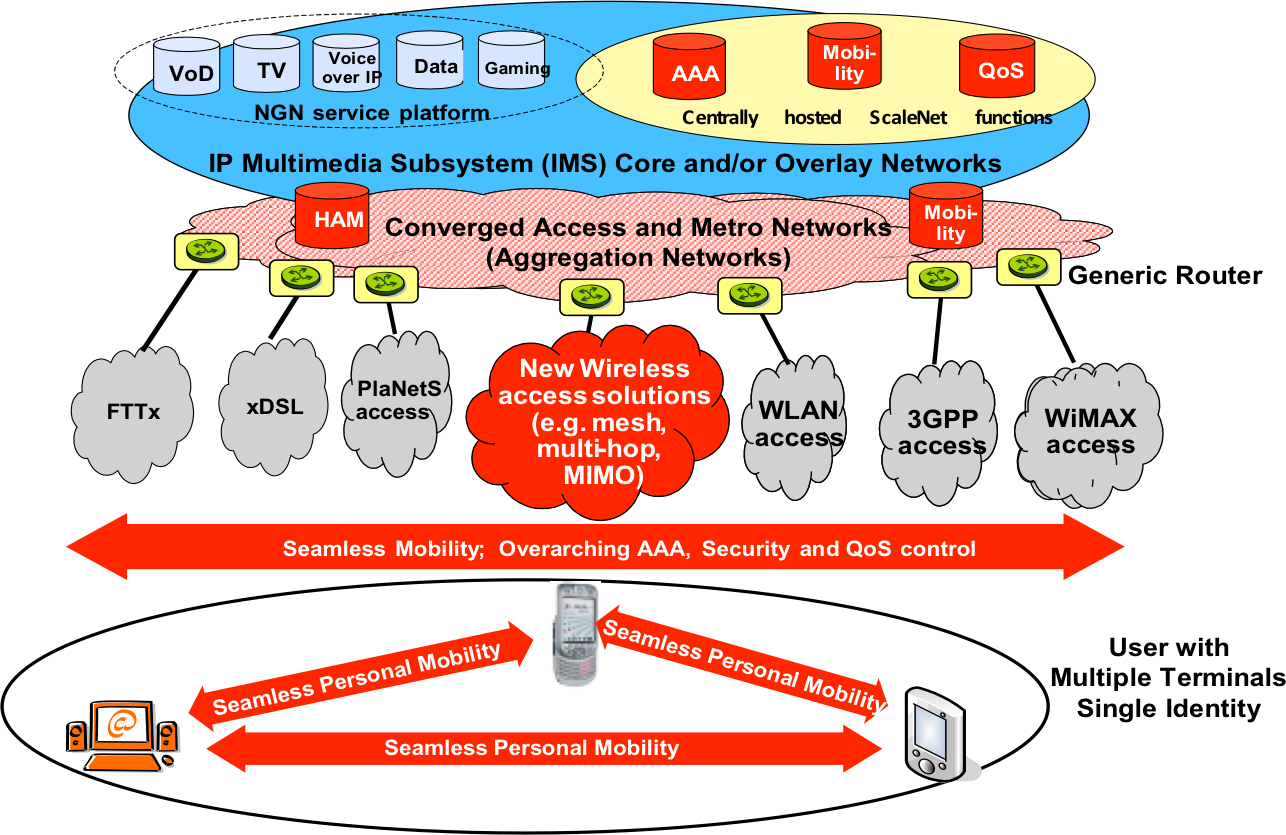
\includegraphics[width=\textwidth]{scalenet-structure}
  \caption{Structure of the system}
  \label{fig:scalenet-structure}
\end{figure}

At an upper level, multimedia services relay on the \ida{IMS} framework for the delivery.
Theoretically \idx{ScaleNet} could support other protocols like Overlay Networks or \ida{P2P}, but \ida{IMS} is the one used by the current implementation.

It is important to notice that the network itself is user-centric, and transparently handles identities by using \ida{SIP}.
This eases supporting users with multiple devices; therefore applications do not have to worry about that part.

It is also important to define what a session means in this system.
A session refers to the current use of a service, so for every service that the user is enjoying a session is created.
For example, if it is viewing a movie but also talking on the \ida{IP} phone, there are two sessions at the same time.

The creation of a session implies that a new service is created, but it goes the other way around too.
If a session is deleted, that service must stop.
If the user ends the service, the session must be deleted.
That means sessions have to be synchronized with the actual services.

A session is also linked to the device that the user is using.
The system allows the copy and transfer of sessions to other devices that he owns, wherever it makes sense.
Since the current implementation has also basic social capabilities, that session can also be transferred or copied to a user's contact.
In the context of this application a user's contact is called ``buddy''.
Figure~\ref{fig:scalenet-structure} lists some of the services that can be offered:

\begin{itemize}
  \item Voice \et{} Video Calls
  \item Mobile TV \et{} \ida{VOD}
  \item \index{MMOG}\acp{MMOG}
  \item Internet Access
\end{itemize}

The work described in this document is primarily focused on the second application, i.e., video streaming.
The idea is that the user can buy a video and play it anywhere using any supported device.

% subsection overviewscalenet (end)
\subsection{\idx{IMS} Demonstrator} % (fold)
\label{sub:demonstrator}

\begin{figure}[htbp]
  \centering
  \subfigure[System architecture]{
    \label{fig:ims-arch}
    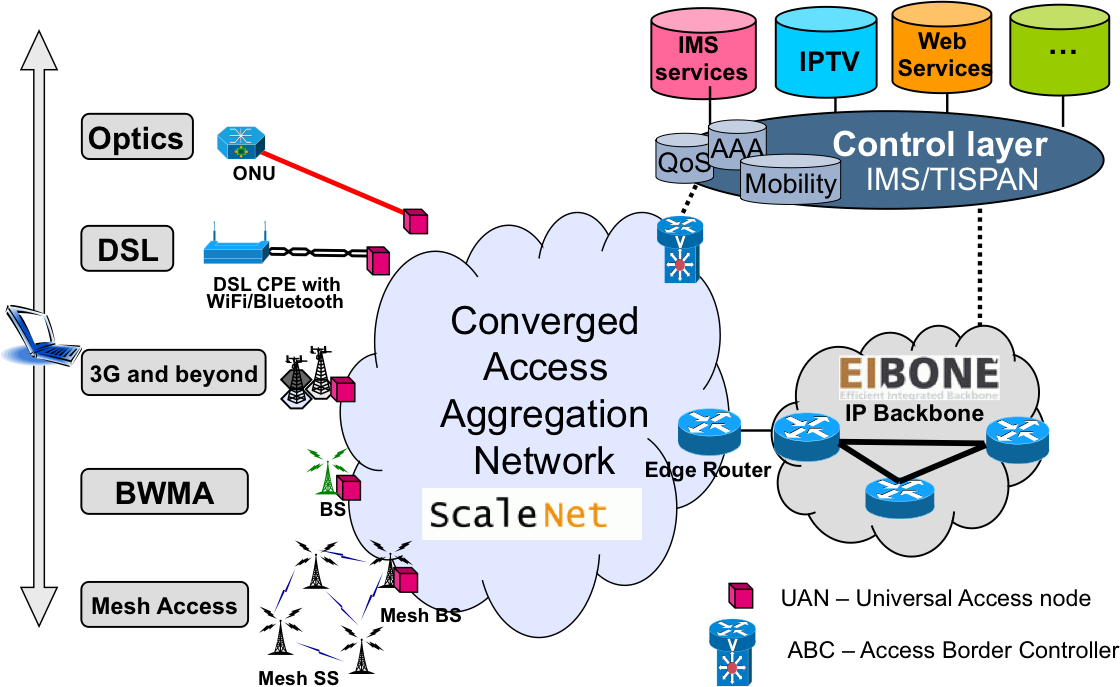
\includegraphics[width=\textwidth]{ims-arch}
  }
  \subfigure[Architecture of the demonstrator]{
    \label{fig:ims-arch-real}
    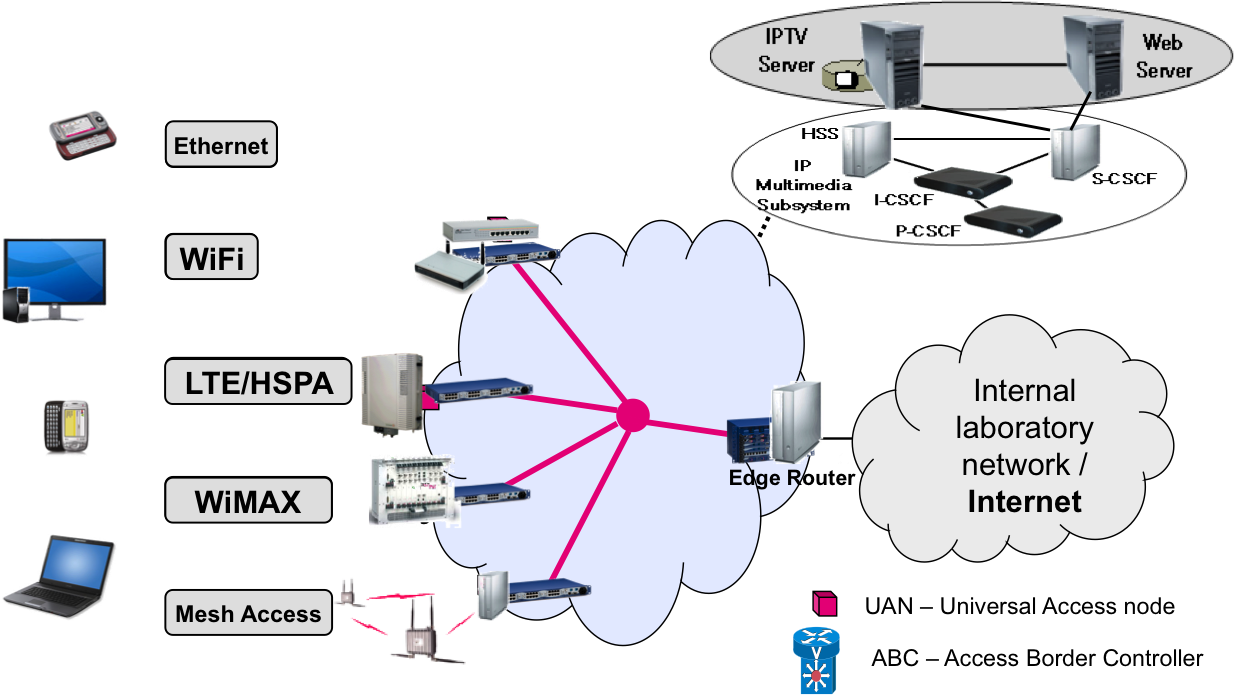
\includegraphics[width=\textwidth]{ims-arch-real}
  }
  \caption{IMS architecture}
  \label{fig:ims}
\end{figure}

A logical view of the system is depicted in Figure~\ref{fig:ims-arch}, explaining the important nodes based on the capabilities needed.
The information relevant to this project is contained in the upper right corner of the figure, the nodes behind the control layer.

In the offices of \ida{T-Labs} in Berlin and Darmstadt there is a demonstrator with a working implementation of \idx{ScaleNet}.
That demonstrator is composed by several servers and a network infrastructure that enables access to the system using different network protocols and devices.
In Figure~\ref{fig:ims-arch-real} the actual network and hardware are exposed, replacing the same space as in the logical view (Figure~\ref{fig:ims-arch}).

\begin{figure}[htbp]
  \centering
    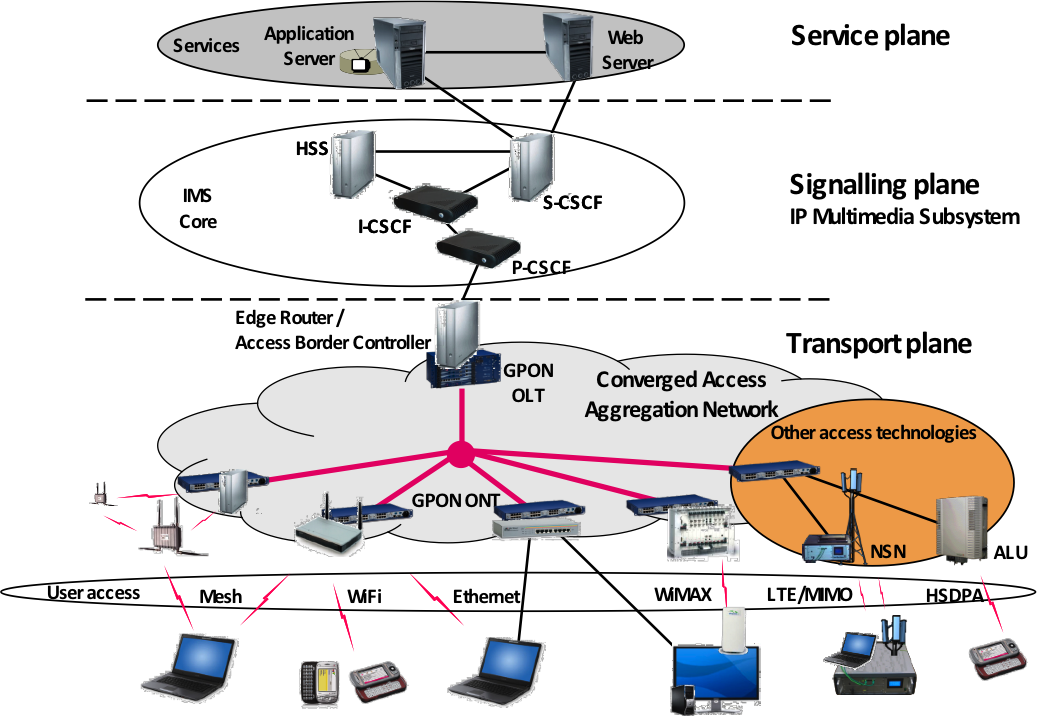
\includegraphics[width=\textwidth]{ims-setup}
  \caption{Setup of the demonstrator}
  \label{fig:ims-setup}
\end{figure}

Figure~\ref{fig:ims-setup} describes the setup in a better way and highlights the three different planes of the demonstrator.
The developed web application is executed from the \idx{Web Server} and the \idx{Application Server}, since it belongs to the service plane.
The signaling plane has also to be taken into account, because it communicates directly with the servers.

However, that is not the real deployment of the hardware used.
Whether for convenience or efficiency, tasks are distributed between two main servers.
This does not affect the logic of the system, since those tasks could be easily decoupled in an alternate deployment with more servers.
Anyway, the interesting pieces of hardware for this project are:

\begin{description}
  \item[\ida{IMS} core] This machine contains the \ida{IMS} server\footnote{The IMS core is open source software from Fraunhofer FOKUS and it can be freely downloaded from: \url{http://www.openimscore.org/}}, but since the \ida{IMS} load is not very high, it is responsible for other things.
  It acts as a \idx{Web Server} (using \idx{Apache} Web Server\footnote{\url{http://httpd.apache.org/}}) serving \ida{PHP} applications.
  It is also the internal \ida{DNS} server.
  \item[\idx{Application Server}] This is the \ida{IPTV} server, where the video content is streamed.
  It is also a \idx{Web Server}, but it serves \idx{Java} applications based on the \ida{OSGi} framework\footnote{\url{http://www.osgi.org/}}.
  \item[User Devices] Devices intended for the user to access the services.
  There is a TV, a laptop and several phones.
  All of them run a custom \ida{IMS} client that holds a connection to the servers, allowing the identification and adding \ida{IPTV} and \ida{VoIP} capabilities to those devices.
  In the last phase of the development, an \idx{iPhone} was added for testing purposes.
\end{description}

This demonstrator contains several demo applications running.
The interesting one for this project is the application that handles \ida{IPTV} streaming.

% subsubsection demonstrator (end)
\subsection{Personal Network Administration Interface (\idx{PNAI})} % (fold)
\label{sub:pnai}

The Web interface used for the management of sessions is called \ida{PNAI}~\cite{SIV08A}. From this interface the user can obtain this information:

\begin{itemize}
  \item All devices and registered in the system for that user and their online status.
  \item All buddies for that user and their online status.
  \item All multimedia sessions related to the user. This includes:
  \begin{itemize}
    \item The sessions running on his devices, no matter who paid for that content.
    \item The sessions running on devices from his buddies and started/paid by that user.
  \end{itemize}
\end{itemize}

Those are passive actions, but from that same view the user can initiate some operations to control the system.
In Figure~\vref{fig:usecasesiptv} all the available operations relating sessions are listed following a use case diagram.

\begin{figure}[htbp]
  \centering
    \includegraphics[width=\textwidth]{diagrams/usecases-pnai-old.1}
  \caption{Use cases for the IPTV application}
  \label{fig:usecasesiptv}
\end{figure}

In that diagram colors are used to differentiate the different kind of use cases covered. Also two visual marks (* and **) are added in case this is a copy in black a white. The meaning of the colors are explained according to this legend:

\begin{description}
  \item[Green] Available already in the main \ida{PNAI} page.
  \item[Purple (\emph{marked with *})] Available in an individual page outside of the main \ida{PNAI} page.
  \item[Red (\emph{marked with **})] Not implemented.
\end{description}

As we can see, the main \ida{PNAI} page has already a lot of functionality, but it can contain even more. Basically the actions available to that user in that page are:

\begin{itemize}
  \item Terminate a session of a user device or of a buddy if the session is owned by that user.
  \item Transfer (handover) or copy (duplication) an existing session to a user device or to a buddy if the session is owned by that user. That is, if one buddy bought the content for us, we cannot transfer again that content to another buddy.
\end{itemize}

Beside of these session related operations, there are other management operations.
For example, selecting which device is the default, adding/removing devices or adding/removing buddies.
For this document they are not relevant since they remained untouched.

Figure~\vref{fig:pnai-old} shows the old appearance of the main page for a logged user, before any work began.
On the left side of the page there is the \idx{Device List}, where the devices owned by that user are drawn.
On the right side there is the \idx{Buddy List}, where the user's buddies are listed.
Finally, the trash bin is in the lower right corner of the \idx{Device List}. 

\begin{figure}[htbp]
  \centering
    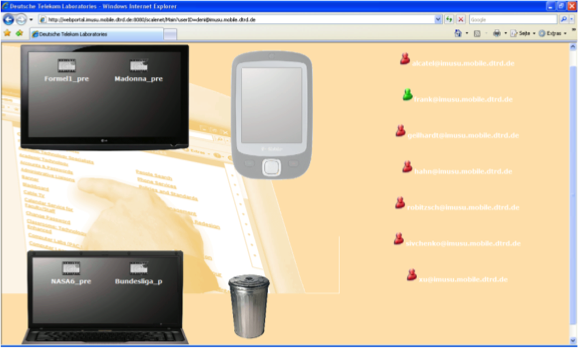
\includegraphics[width=\textwidth]{pnai-old}
  \caption{Old \idx{PNAI} page}
  \label{fig:pnai-old}
\end{figure}

The devices that are offline are disabled and are drawn with a dimmed appearance.
The buddies that are online are preceded by a green icon, while the ones that are offline are preceded by a red icon.

Devices or buddies that are online act as session containers.
The reason for the devices to be so big is because inside them the current sessions are drawn.
Besides the name of the content playing, session have an icon that changes depending on the type of session (video, audio, call, etc).

The user can interact with the sessions through the mouse using \idx{drag\et{}drop}.
For example, the user can \emph{grab} the icon he wants and drop it in another container to copy or transfer that session.
That is a very visual and fast way to manage sessions.

When a user drops the session in another container, a menu will appear to ask the user if he wants to copy or transfer that session.
The trash bin acts also as a container, but in a special way: when a session is dropped in the trash bin, that session is automatically deleted, with no menu involved.

\subsubsection{Use Cases} % (fold)
\label{ssub:usecasesold}

In the following tables the current supported use cases are explained step by step.
The first use case is detailed in Table~\vref{tab:usecasestopdevice}, explaining the situation where the user wants to stop/delete the session in a device.

\begin{center}
  \begin{usecase}[Stop a session of a device]
    \label{tab:usecasestopdevice}%
    \usecaseactor{System user}
    \usecasepre{A session is already running on a device, and it is showing in the \ida{PNAI} interface inside of that device.}
    \usecasepost{Session must terminate, i.e., the content must stop playing. The user must be notified with a popup and the session icon must be deleted from the \ida{PNAI} interface.}
    \usecasemain{
      \begin{usecasepath}
        \item User starts dragging the session icon.
        \item A copy of the session icon appears under the user's cursor, and follows the cursor until the user drops it.
        \item User drops the cloned session icon into the trash.
        \item A popup appears to notify the user that the action is in progress and the cloned session icon is deleted from the view.
        \item The content stops playing.
        \item The popup disappears and the original session icon is deleted from the view.
      \end{usecasepath}
    }
    \usecasealt{1}{
      \begin{usecasepath}[b]
        \setcounter{enumi}{2}
        \item User drops the session into a blank space.
        \item Action is cancelled.
      \end{usecasepath}
    }
    \usecasealt{2}{
      \begin{usecasepath}[c]
        \setcounter{enumi}{4}
        \item There is an error with the server and the content keeps playing.
        \item The content of the popup changes to notify the user that there was an error with the server and the action could not be completed.
        After 5 seconds it disappears.
        \item Action is cancelled.
      \end{usecasepath}
    }
  \end{usecase}
\end{center}

\begin{figure}[htbp]
  \centering
    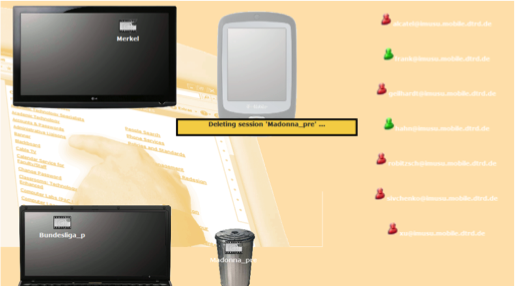
\includegraphics[width=\textwidth]{pnai-old-stop}
  \caption{Deleting a session in the old \idx{PNAI}}
  \label{fig:pnai-old-stop}
\end{figure}

Figure~\vref{fig:pnai-old-stop} shows how the page looks when it is waiting for a response to the server for the previous use case.
Since the user interface does not block in the process, the communication between the front end and the back end must be asynchronous.
The use case for terminating a session that a buddy is playing and that we own is very similar, as Table~\vref{tab:usecasestopbuddy} exposes.

\begin{center}
  \begin{usecase}[Stop a session of a buddy]
    \label{tab:usecasestopbuddy}%
    \usecaseactor{System user}
    \usecasepre{A session owned by the user is running on a device, and it is showing in the \ida{PNAI} interface near that buddy's name.}
    \usecasepost{Session must terminate, i.e., the content must stop playing. The user must be notified with a popup and the session icon must be deleted from the \ida{PNAI} interface. The buddy is \emph{not} notified, the content stops without warning.}
    \usecasemain{
      \begin{usecasepath}
        \item User starts dragging the session icon.
        \item A copy of the session icon appears under the user's cursor, and follows the cursor until the user drops it.
        \item User drops the cloned session icon into the trash.
        \item A popup appears to notify the user that the action is in progress and the cloned session icon is deleted from the view.
        \item The content stops playing.
        \item The popup disappears and the original session icon is deleted from the view.
      \end{usecasepath}
    }
    \usecasealt{1}{
      \begin{usecasepath}[b]
        \setcounter{enumi}{2}
        \item User drops the session into a blank space.
        \item Action is cancelled.
      \end{usecasepath}
    }
    \usecasealt{2}{
      \begin{usecasepath}[c]
        \setcounter{enumi}{4}
        \item There is an error with the server and the content keeps playing.
        \item The content of the popup changes to notify the user that there was an error with the server and the action could not be completed.
        After 5 seconds it disappears.
        \item Action is cancelled.
      \end{usecasepath}
    }
  \end{usecase}
\end{center}

Tables~\vref{tab:usecasecopydevice},~\vref{tab:usecasecopybuddy},~\vref{tab:usecasetransferdevice}~and~\vref{tab:usecasetransferbuddy} show how the user could copy or transfer a session to another device or buddy.

\begin{center}
  \begin{usecase}[Copy a session to a device]
    \label{tab:usecasecopydevice}%
    \usecaseactor{System user}
    \usecasepre{A session is already running on a device/buddy, and it is showing in the \ida{PNAI} interface inside of that device/buddy. Also, there is another device online.}
    \usecasepost{Session must be copied to that device, i.e., the content must be duplicated and played on that device. The user must be notified with a popup and the session icon must appear in the \ida{PNAI} interface for the second device.}
    \usecasemain{
      \begin{usecasepath}
        \item User starts dragging the session icon.
        \item A copy of the session icon appears under the user's cursor, and follows the cursor until the user drops it.
        \item User drops the cloned session icon into another device that is online.
        \item A popup menu appears where the user dropped the session, giving options to copy/duplicate the session, transfer the session or cancel the action.
        \item The user clicks on the copy/duplicate option.
        \item The popup menu disappears.
        \item A popup appears to notify the user that the action is in progress and the cloned session icon is deleted from the view.
        \item The content starts playing on the destination device.
        \item The popup disappears and the same session icon appears inside of the destination device.
      \end{usecasepath}
    }
    \usecasealt{1}{
      \begin{usecasepath}[b]
        \setcounter{enumi}{2}
        \item User drops the session into a blank space.
        \item Action is cancelled.
      \end{usecasepath}
    }
    \usecasealt{2}{
      \begin{usecasepath}[c]
        \setcounter{enumi}{4}
        \item The user clicks on the cancel option.
        \item Popup menu disappears and action is cancelled.
      \end{usecasepath}
    }
    \usecasealt{3}{
      \begin{usecasepath}[d]
        \setcounter{enumi}{7}
        \item There is an error with the server and the content is not duplicated.
        \item The content of the popup changes to notify the user that there was an error with the server and the action could not be completed.
        After 5 seconds it disappears.
        \item Action is cancelled.
      \end{usecasepath}
    }
  \end{usecase}
\end{center}

\begin{center}
  \begin{usecase}[Copy a session to a buddy]
    \label{tab:usecasecopybuddy}%
    \usecaseactor{System user}
    \usecasepre{A session is already running on a device/buddy, and it is showing in the \ida{PNAI} interface inside of that device/buddy. Also, there is another buddy online.}
    \usecasepost{Session must be copied to that buddy, i.e., the content must be duplicated and played on the buddy's default device. The user must be notified with a popup and the session icon must appear in the \ida{PNAI} interface near the name of that buddy. The buddy is \emph{not} notified, the content plays without warning.}
    \usecasemain{
      \begin{usecasepath}
        \item User starts dragging the session icon.
        \item A copy of the session icon appears under the user's cursor, and follows the cursor until the user drops it.
        \item User drops the cloned session icon into another buddy that is online.
        \item A popup menu appears where the user dropped the session, giving options to copy/duplicate the session, transfer the session or cancel the action.
        \item The user clicks on the copy/duplicate option.
        \item The popup menu disappears.
        \item A popup appears to notify the user that the action is in progress and the cloned session icon is deleted from the view.
        \item The content starts playing on the buddy's default device.
        \item The popup disappears and the same session icon appears inside of the destination buddy.
      \end{usecasepath}
    }
    \usecasealt{1}{
      \begin{usecasepath}[b]
        \setcounter{enumi}{2}
        \item User drops the session into a blank space.
        \item Action is cancelled.
      \end{usecasepath}
    }
    \usecasealt{2}{
      \begin{usecasepath}[c]
        \setcounter{enumi}{4}
        \item The user clicks on the cancel option.
        \item Popup menu disappears and action is cancelled.
      \end{usecasepath}
    }
    \usecasealt{3}{
      \begin{usecasepath}[d]
        \setcounter{enumi}{7}
        \item There is an error with the server and the content is not duplicated.
        \item The content of the popup changes to notify the user that there was an error with the server and the action could not be completed.
        After 5 seconds it disappears.
        \item Action is cancelled.
      \end{usecasepath}
    }
  \end{usecase}
\end{center}

\begin{center}
  \begin{usecase}[Transfer a session to a device]
    \label{tab:usecasetransferdevice}%
    \usecaseactor{System user}
    \usecasepre{A session is already running on a device/buddy, and it is showing in the \ida{PNAI} interface inside of that device/buddy. Also, there is another device online.}
    \usecasepost{Session must be transferred to that device, i.e., playback must be stopped at the source and started at the destination device. The user must be notified with a popup and the session icon must appear in the \ida{PNAI} interface for the second device.}
    \usecasemain{
      \begin{usecasepath}
        \item User starts dragging the session icon.
        \item A copy of the session icon appears under the user's cursor, and follows the cursor until the user drops it.
        \item User drops the cloned session icon into another device that is online.
        \item A popup menu appears where the user dropped the session, giving options to copy the session, transfer/hand over the session or cancel the action.
        \item The user clicks on the transfer/hand over option.
        \item The popup menu disappears.
        \item A popup appears to notify the user that the action is in progress and the cloned session icon is deleted from the view.
        \item The content stops playing on the source device.
        \item The content starts playing on the destination device.
        \item The popup disappears, the session icon is deleted from the view and created again inside of the destination device.
      \end{usecasepath}
    }
    \usecasealt{1}{
      \begin{usecasepath}[b]
        \setcounter{enumi}{2}
        \item User drops the session into a blank space.
        \item Action is cancelled.
      \end{usecasepath}
    }
    \usecasealt{2}{
      \begin{usecasepath}[c]
        \setcounter{enumi}{4}
        \item The user clicks on the cancel option.
        \item Popup menu disappears and action is cancelled.
      \end{usecasepath}
    }
    \usecasealt{3}{
      \begin{usecasepath}[d]
        \setcounter{enumi}{7}
        \item There is an error with the server and the content is not transferred.
        \item The content of the popup changes to notify the user that there was an error with the server and the action could not be completed.
        After 5 seconds it disappears.
        \item Action is cancelled.
      \end{usecasepath}
    }
  \end{usecase}
\end{center}

\begin{center}
  \begin{usecase}[Transfer a session to a buddy]
    \label{tab:usecasetransferbuddy}%
    \usecaseactor{System user}
    \usecasepre{A session is already running on a device/buddy, and it is showing in the \ida{PNAI} interface inside of that device/buddy. Also, there is another buddy online.}
    \usecasepost{Session must be transferred to that buddy, i.e., playback must be stopped at the source and started at the buddy's default device. The user must be notified with a popup and the session icon must appear in the \ida{PNAI} interface near the name of that buddy. The buddy is \emph{not} notified, the content plays without warning.}
    \usecasemain{
      \begin{usecasepath}
        \item User starts dragging the session icon.
        \item A copy of the session icon appears under the user's cursor, and follows the cursor until the user drops it.
        \item User drops the cloned session icon into another buddy that is online.
        \item A popup menu appears where the user dropped the session, giving options to copy the session, transfer/hand over the session or cancel the action.
        \item The user clicks on the transfer/hand over option.
        \item The popup menu disappears.
        \item A popup appears to notify the user that the action is in progress and the cloned session icon is deleted from the view.
        \item The content stops playing on the source device.
        \item The content starts playing on the buddy's default device.
        \item The popup disappears, the session icon is deleted from the view and created again inside of the destination buddy.
      \end{usecasepath}
    }
    \usecasealt{1}{
      \begin{usecasepath}[b]
        \setcounter{enumi}{2}
        \item User drops the session into a blank space.
        \item Action is cancelled.
      \end{usecasepath}
    }
    \usecasealt{2}{
      \begin{usecasepath}[c]
        \setcounter{enumi}{4}
        \item The user clicks on the cancel option.
        \item Popup menu disappears and action is cancelled.
      \end{usecasepath}
    }
    \usecasealt{3}{
      \begin{usecasepath}[d]
        \setcounter{enumi}{7}
        \item There is an error with the server and the content is not transferred.
        \item The content of the popup changes to notify the user that there was an error with the server and the action could not be completed.
        After 5 seconds it disappears.
        \item Action is cancelled.
      \end{usecasepath}
    }
  \end{usecase}
\end{center}

\begin{figure}[htbp]
  \centering
    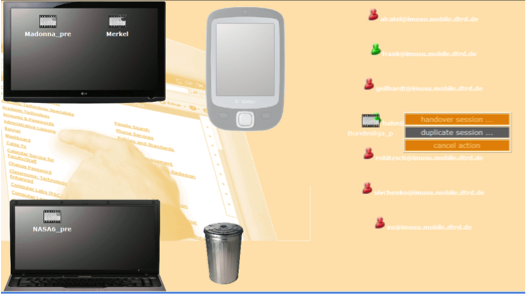
\includegraphics[width=\textwidth]{pnai-old-duplicate}
  \caption{Duplicating a session in the old \idx{PNAI}}
  \label{fig:pnai-old-duplicate}
\end{figure}

Figure~\vref{fig:pnai-old-duplicate} shows how the popup menu is displayed to the user.
It is a very simple menu with only three links, each of which correspond to an action.

% subsubsection usecasesold (end)
\subsubsection{Components} % (fold)
\label{ssub:componentsold}

As explained in \S\ref{sub:demonstrator}, the software is mainly executed in three machines: two servers and a client.
Figure~\ref{fig:componentdiagramsold} shows all the relevant components running inside those machines and how they interact with each other.

\begin{figure}[htbp]
  \centering
    \includegraphics[width=\textwidth]{diagrams/component-pnai-old.1}
  \caption{Component diagram for the old \idx{PNAI}}
  \label{fig:componentdiagramsold}
\end{figure}

That component diagram brings some interesting aspects about the system, although we are only interested in several of them:

\begin{itemize}
  \item The \ida{SIP} protocol is used for the IMS part, but this is not important for the work done, as both the server and the client were not touched.
  \item The \ida{SSCON} manages the sessions and acts as the bridge between the actual services and the web interface shown to the user.
  Actions from the web interface are notified through \ida{UDP} calls.
  \item In this diagram, though, there are two parts missing that are almost completely irrelevant for this document.
  These are the application server component that streams the content and the multimedia player installed in the user device.
  The protocols used between these two components are not interesting for us, so for sake of simplicity, they don't appear here.
  The only important thing is that the \ida{SIP} client controls the external player, so the web interface does not handle the video streaming.
  \item There are two MySQL databases in use:
  \begin{description}
    \item[\idx{HSS DB}] This is the master database, and it is always up to date.
    It contains information about the user status, his buddy list and registered devices.
    \item[\idx{Personal DB}] This is an additional database that depends on the HSS DB.
    This database gather all the information needed for the \ida{PNAI}, since it contains all the relevant information from the \idx{HSS DB} plus the session information obtained from the \ida{SSCON}.
    Periodically, the \ida{SSCON} polls information from the master database and then updates this slave database, so the information can be a bit outdated compared to the \idx{HSS DB}.
    As stated in the diagram, the \ida{OSGi} component grabs the information it needs from this database, by polling it periodically.
  \end{description}
  \item Once the page is sent to the browser, the web interface continues talking with the server through a \ida{TCP} socket without reloading the page.
  This goes both ways, since it is used for sending actions and receiving data following a push model (so no delays polling).
  Since, at the time of developing the original application, there was no way to get that using only basic web standards, it uses a \idx{Java applet} to handle the socket communications.
\end{itemize}

\begin{figure}[htbp]
  \centering
    \includegraphics[width=\textwidth]{diagrams/sequence-handover-old.1}
  \caption{Sequence diagram for the old \idx{PNAI}}
  \label{fig:sequence-handover-old}
\end{figure}

Figure~\ref{fig:sequence-handover-old} shows the flow of the application in the scenario where the user wants to transfer a session from his device to one of those buddies.
Blue lines belong to the main logical flow, while the yellow ones belong to the video streaming process.
Other usage scenarios are very similar to this one, so they are ignored since this one explains well how and when they communicate.

As we can see, the web interface (written in \idx{JavaScript}) talks back and forth with the \idx{Java applet} using simple method calls, since all the code interface are directly available between them.
Then the \idx{Java applet} translates those calls to strings with the method names and parameters and sends it to the \ida{OSGi} using the \ida{TCP} connection.

At the right part of the diagram, it is clear that the sessions are controlled using \ida{SIP} messages.
Given that \idx{ScaleNet} is a very decentralized network by design, the \ida{SSCON} delegates to the \ida{SIP} clients running in the devices all the talking with the \idx{Application Server}.

It is interesting to note that everything is mostly asynchronous, so there is not a lot of calls that block.
Therefore the use of threads and callbacks is widespread in all components.

% subsubsection componentsold (end)
\subsubsection{Personal DB} % (fold)
\label{ssub:personaldb}

The database that is directly used by the \ida{PNAI} is the \idx{Personal DB}. The most important table is the \idc{current\_session} table, where is all the information about the sessions that are currently active.
Table~\vref{tab:sessiondb} explains all the fields in this table, and Table~\vref{tab:sessiondbexample} details an example entry.

\begin{generictable}[Current session table architecture]{2}
  {|p{0.21\textwidth}|p{0.69\textwidth}|}
  {\generictitletwo{Field name}{Description}}
  \label{tab:sessiondb}%
  \idc{id} & Identifier, auto-increment integer \\ \hline
  \idc{impi} & Private identity of user \\ \hline
  \idc{impu} & Public identity of user \\ \hline
  \idc{callid} & Unique number to identify session details \\ \hline
  \idc{partner} & Next party of session (AS identity if client to AS or impu of partner if client to client) \\ \hline
  \idc{as} & \idx{Application Server} identity (client to AS) or NULL (client to client) \\ \hline
  \idc{ip} & \ida{IP} address for impu \\ \hline
  \idc{initiator} & impu who sends the INVITE message \\ \hline
  \idc{owner} & impi who needs to pay for the session. Usually the impi who sends the \idc{invite} message, but it can be the impi who sends the \idc{refer} message in case of transfer/duplication \\ \hline
  \idc{session\_name} & Name of the session \\ \hline
  \idc{type} & Type of the session (audio/video) \\ \hline
  \idc{bw} & Bandwidth of the session \\ \hline
  \idc{source} & \ida{URL} of the source \\ \hline
  \idc{lov} & Type of video transmission (live/video on demand/tv)\\ \hline
  \idc{cid}/\idc{did}/\idc{tid} & Integers related to \ida{QoS} parameters \\ \hline
  \idc{session\_flag} &
  0 if it is a normal session \newline
  1 if it is a transferred session \newline
  2 if it is a duplicated session
  \\ \hline
\end{generictable}

\begin{generictable}[Current session table example]{2}
  {|p{0.21\textwidth}|p{0.69\textwidth}|}
  {\generictitletwo{Field name}{Example value}}
  \label{tab:sessiondbexample}%
  \idc{id} & 3 \\ \hline
  \idc{impi} & deni@imusu.mobile.dtrd.de \\ \hline
  \idc{impu} & mda.deni@imusu.mobile.dtrd.de \\ \hline
  \idc{callid} & 783457644 \\ \hline
  \idc{partner} & as@imusu.mobile.dtrd.de or tv.hahn@imusu.mobile.dtrd.de \\ \hline
  \idc{as} & as@imusu.mobile.dtrd.de \\ \hline
  \idc{ip} & 19.168.5.92 \\ \hline
  \idc{initiator} & mda.deni@imusu.mobile.dtrd.de or as@imusu.mobile.dtrd.de \\ \hline
  \idc{owner} & deni@imusu.mobile.dtrd.de \\ \hline
  \idc{session\_name} & NASA \\ \hline
  \idc{type} & video \\ \hline
  \idc{bw} & 5000 \\ \hline
  \idc{source} & http://appserver:9000 \\ \hline
  \idc{lov} & video on demand\\ \hline
  \idc{cid}/\idc{did}/\idc{tid} & 3/5/12 \\ \hline
  \idc{session\_flag} & 0 \\ \hline
\end{generictable}

Other important table is the \idc{user\_status} table, that lists all the users in the system and some basic information about them.
Table~\vref{tab:userdb} explains all the fields in this table, and Table~\vref{tab:userdbexample} details an example entry.

\begin{generictable}[User status table architecture]{2}
  {|p{0.21\textwidth}|p{0.69\textwidth}|}
  {\generictitletwo{Field name}{Description}}
  \label{tab:userdb}%
  \idc{id} & Identifier, auto-increment integer \\ \hline
  \idc{impi} & Private identity of user \\ \hline
  \idc{impu} & Public identity of user \\ \hline
  \idc{impi\_id} & Unique id to identify impi \\ \hline
  \idc{impu\_id} & Unique id to identify impu \\ \hline
  \idc{status} & Status of impu: 1 (online), 0 (offline) \\ \hline
\end{generictable}

\begin{generictable}[User status table example]{2}
  {|p{0.21\textwidth}|p{0.69\textwidth}|}
  {\generictitletwo{Field name}{Example value}}
  \label{tab:userdbexample}%
  \idc{id} & 1 \\ \hline
  \idc{impi} & deni@imusu.mobile.dtrd.de \\ \hline
  \idc{impu} & laptop.deni@imusu.mobile.dtrd.de \\ \hline
  \idc{impi\_id} & 67 \\ \hline
  \idc{impu\_id} & 35 \\ \hline
  \idc{status} & 1 \\ \hline
\end{generictable}

Finally, there is a third table that handles the relationships between friends called \idc{web\_buddylist}.
It is a very simple table modeling a classic many-to-many relationship, but anyway Table~\vref{tab:buddydb} explains all its fields, and Table~\vref{tab:buddydbexample} details an example entry.

\begin{generictable}[Buddy list table architecture]{2}
  {|p{0.2\textwidth}|p{0.69\textwidth}|}
  {\generictitletwo{Field name}{Description}}
  \label{tab:buddydb}%
  \idc{id} & Identifier, auto-increment integer \\ \hline
  \idc{impi\_id} & Unique id to identify impi (identical to impi\_id of \idc{user\_status} table) \\ \hline
  \idc{buddy\_impi\_id} & Unique id to identify the buddy impi \\ \hline
\end{generictable}

\begin{generictable}[Buddy list table example]{2}
  {|p{0.21\textwidth}|p{0.69\textwidth}|}
  {\generictitletwo{Field name}{Example value}}
  \label{tab:buddydbexample}%
  \idc{id} & 2 \\ \hline
  \idc{impi\_id} & 56 \\ \hline
  \idc{buddy\_impi\_id} & 67 \\ \hline
\end{generictable}

These tables are not changed during the development explained in this document, neither the software that access those tables directly.
However, it is interesting to know the kind of data they have because indirectly it is the same data we are going to process.

% subsubsection personaldb (end)
\subsubsection{Messages} % (fold)
\label{ssub:messagesold}

Of all the messages sent inside the system, the most important ones for us are sent though the \ida{TCP} socket.
These are processed and generated by the web interface and the \ida{OSGi} backend, but they follow a different format depending which component sends the message.

Messages generated by the backend consist of serialized objects following a very simple format.
There are three kind of data objects that can be sent over the wire: devices, buddies and sessions.

A serialized object is a string that starts with the type of the object (\idc{device}, \idc{buddy}, \idc{session}), followed by the vertical bar character `|' as delimiter.
Then the attributes for that object are appended one by one, separated by the same delimiter.
If the values are not strings, they are converted directly, for example a boolean with value \texttt{true} will be passed as the string \texttt{"true"}.

The client does not know when a transfer or duplication happens, it is only notified of creation and deletion of things.
When a status update happens, such as a device going online, it is notified as the creation of an object.
Therefore the client must keep track of the objects received and realize that it is an update of a previously created object.

For example, as seen in Figure~\vref{fig:sequence-handover-old}, when a transfer happens the interface received two commands, first creating a new session and then deleting the original session.

To notify that a new object needs to be created in the view, the backend just sends the serialized object, without adding anything else.
To notify that an existing object has to be deleted from the view, the string is the same but preceded by the text \texttt{"deleted|"} (that is, \emph{deleted} and the delimiter).

Table~\vref{tab:notificationsexamples} comprises all the different messages that can be sent from the \ida{OSGi} backend to the \idx{Java applet} with examples.

\begin{generictable}[Format of the notifications sent to the applet]{2}
  {|p{0.21\textwidth}|p{0.69\textwidth}|}
  {\generictitletwo{Notification}{Format \et{} Example}}
  \label{tab:notificationsexamples}%
  Create/update device & \texttt{device|\emph{impi}|\emph{impu}|\emph{online}} \newline
    \texttt{device|hahn@imusu.mobile.dtrd.de\newline
    $\hookrightarrow$|tv.hahn@imusu.mobile.drtd.de|true} \\ \hline
  Delete device & \texttt{deleted|device|\emph{impi}|\emph{impu}|%
    \emph{online}} \newline
    \texttt{deleted|device|hahn@imusu.mobile.dtrd.de\newline
    $\hookrightarrow$|tv.hahn@imusu.mobile.drtd.de|false} \\ \hline
  Create/update buddy & \texttt{buddy|\emph{id}|\emph{name}|\emph{online}}%
    \newline
    \texttt{buddy|3|hahn@imusu.mobile.dtrd.de|false} \\ \hline
  Delete buddy & \texttt{deleted|buddy|\emph{id}|\emph{name}|\emph{online}}%
    \newline
    \texttt{deleted|buddy|3|hahn@imusu.mobile.dtrd.de\newline
    $\hookrightarrow$|false} \\ \hline
  Create/update session & \texttt{session|\emph{id}|\emph{type}|\emph{name}%
    |\emph{owner}|\emph{initiator}|\emph{impi}\newline
    $\hookrightarrow$|\emph{impu}|\emph{icon}}
    \newline
    \texttt{session|3|video|NASA\newline
    $\hookrightarrow$|hahn@imusu.mobile.dtrd.de\newline
    $\hookrightarrow$|hahn@imusu.mobile.dtrd.de\newline
    $\hookrightarrow$|hahn@imusu.mobile.dtrd.de\newline
    $\hookrightarrow$|laptop.hahn@imusu.mobile.dtrd.de\newline
    $\hookrightarrow$|http://imusu.mobile.dtrd.de/img/icon.png} \\ \hline
  Delete session & \texttt{deleted|session|\emph{id}|\emph{type}|\emph{name}%
    |\emph{owner}\newline
    $\hookrightarrow$|\emph{initiator}|\emph{impi}|\emph{impu}|\emph{icon}}
    \newline
    \texttt{deleted|session|3|video|NASA\newline
    $\hookrightarrow$|hahn@imusu.mobile.dtrd.de\newline
    $\hookrightarrow$|hahn@imusu.mobile.dtrd.de\newline
    $\hookrightarrow$|hahn@imusu.mobile.dtrd.de\newline
    $\hookrightarrow$|laptop.hahn@imusu.mobile.dtrd.de\newline
    $\hookrightarrow$|http://imusu.mobile.dtrd.de/img/icon.png} \\ \hline
\end{generictable}

Going back to Figure~\vref{fig:sequence-handover-old}, the message sent in \texttt{TCP(2)} was a \emph{Create/Update session} notification, while the message sent in \texttt{TCP(2)} was a \emph{Delete session} notification.
In both cases, the \idx{Java applet} just parsed the messages and passed the arguments to the right \idx{JavaScript} callbacks.

On the other hand, messages sent by the \idx{Java applet} are requests from the user, for actions that he wants to complete relating sessions.
These actions can be the deletion of a session, its transfer or its duplication.

It does not matter which kind of origin (device or buddy) or destination it goes, because dealing with unique \ida{SIP} identifiers (\idc{impi}) makes sure that every element is treated equally.

They follow a query string format, which is the usual way to pass data as part of a \ida{URL}.
This string is passed directly to the \ida{TCP} socket, without any additional encoding.

Table~\vref{tab:requestsexamples} lists the different messages that can be sent from the \idx{Java applet} to the \ida{OSGi} backend with examples.

\begin{generictable}[Format of the requests sent from the applet]{2}
  {|p{0.21\textwidth}|p{0.69\textwidth}|}
  {\generictitletwo{Request}{Format \et{} Example}}
  \label{tab:requestsexamples}%
  Copy session & \texttt{event=duplicate\&uid=\emph{uid}\&%
    source=\emph{source}\newline
    $\hookrightarrow$\&sid=\emph{sid}\&destination=\emph{target}}\newline
    \texttt{event=duplicate\newline
    $\hookrightarrow$\&uid=hahn@imusu.mobile.dtrd.de\newline
    $\hookrightarrow$\&source=laptop.hahn@imusu.mobile.drtd.de\newline
    $\hookrightarrow$\&sid=458215\newline
    $\hookrightarrow$\&destination=steffen@imusu.mobile.drtd.de} \\ \hline
  Transfer session & \texttt{event=handover\&uid=\emph{uid}\&%
    source=\emph{source}\newline
    $\hookrightarrow$\&sid=\emph{sid}\&destination=\emph{target}}\newline
    \texttt{event=handover\newline
    $\hookrightarrow$\&uid=hahn@imusu.mobile.dtrd.de\newline
    $\hookrightarrow$\&source=laptop.hahn@imusu.mobile.drtd.de\newline
    $\hookrightarrow$\&sid=458215\newline
    $\hookrightarrow$\&destination=tv.hahn@imusu.mobile.drtd.de} \\ \hline
  Stop session & \texttt{event=delete\&uid=\emph{uid}\&%
    source=\emph{source}\&sid=\emph{sid}}\newline
    \texttt{event=delete\&uid=hahn@imusu.mobile.dtrd.de\newline
    $\hookrightarrow$\&source=laptop.hahn@imusu.mobile.drtd.de\newline
    $\hookrightarrow$\&sid=458215} \\ \hline
\end{generictable}

\texttt{TCP(1)} in Figure~\vref{fig:sequence-handover-old} is a typical \emph{Transfer session} request, generated by a \idx{Java applet} after the \idx{JavaScript} requested it upon a user's action.
Additionally, \texttt{UDP(1)} follows the same format and \texttt{SIP(1)} contains the same information but in \ida{SIP} format.
Other messages from that figure are not explained with more detail because the pieces of code that deal with MySQL or SIP are in other modules apart from the web application.

% subsubsection messagesold (end)
\subsubsection{Java Applet Codebase} % (fold)
\label{ssub:appletcodeold}

The same codebase (classes, resources, etc.) is shared between the \ida{OSGi} backend and the \idx{Java applet}, taking advantage of the fact that they are written in the same language.
Though this does not mean that the final executables are the same, since two bundles are generated, one for each purpose.
More details about how \ida{OSGi} and \idx{Java applet}s work in general are discussed on \S\ref{sec:java}.

\begin{figure}[htbp]
  \centering
    \includegraphics[width=\textwidth]{diagrams/class-pnai-java-old.1}
  \caption{Class diagram for the \idx{Java applet}}
  \label{fig:class-pnai-java-old}
\end{figure}

Figure~\ref{fig:class-pnai-java-old} shows all the packages involved in the \idx{Java applet}.
All classes exclusively related to the \ida{OSGi} backend are ignored, since they are not important for this work.

This diagram contains two packages: \idc{Applet} and \idc{Model}.
The first one encloses all the logic needed to contact the socket in the backend (\idc{BackendLink}), and the \idx{Java applet} itself with the interface available to the \idx{JavaScript} codebase (\idc{ScalenetApplet}).

From those classes it is easy to identify the three external parameters needed by the \idx{Java applet}: the user identifier (\ida{SIP} format, email-like), and hostname and port used by the backend (where the socket is reached).

The \idc{Model} package, shared with the backend codebase, comprises all the data model objects.
This includes utilities to create objects from strings, following the formats explained in Tables~\ref{tab:notificationsexamples} and \ref{tab:requestsexamples}.
The attributes for each class object are the same used in those tables.

To create a \idc{Buddy}, \idc{Device} or \idc{Session}, a factory pattern is used, calling the static method \idc{fromString}\footnote{For technical reasons the method \idc{fromString} could not be underlined in the diagram, as the \idas{UML} specification recommends for static methods/attributes.
To bring attention to this important quirk, the method's name is surrounded by underscores.} of the class we want to create an object from.
For some reason, to create a \idc{Request} first the object is created and then the string is parsed to fill all the attributes.
In any case a string is the preferred way to specify the attributes of an object.

% subsubsection appletcodeold (end)
\subsubsection{JavaScript Codebase} % (fold)
\label{ssub:jscodeold}

Finally, we get to the old \idx{JavaScript} codebase, the main place where the effort of this work was focused.
The code resides in the resources folder of the \ida{OSGi} bundle, where all the static public code is thrown: \idas{HTML}, \idas{CSS}, \idx{JavaScript}, images, etc.
When requested by a browser, these files are served by the \ida{OSGi}-based server, not \idx{Apache}.

\idx{JavaScript} classes are organized in several source files, each file acting as if they were traditional packages.
As discussed on \S~\ref{sec:javascript}, \emph{class} is not the right term to refer to a \idx{JavaScript} object, but it will be used through this document for simplicity's sake.

Additionally, in the old codebase the use of global variables is wildly used, and they are quite important to understand how the application works.
Since the \ida{UML} language is designed for \ida{OOP}, there is no easy solution to specify those variables in the same diagram.
However, a workaround is to directly copy how the \ida{DOM} works and put all those variables under the global \idc{window} object.

Figure~\ref{fig:class-pnai-js-old} shows a diagram with all the classes involved and the relationships between them.
Figure~\ref{fig:class-pnai-global-old} completes the picture adding the global object and the relationships between it and the custom classes.

\begin{figure}[htbp]
  \centering
    \includegraphics[width=\textwidth]{diagrams/class-pnai-js-old.1}
  \caption{Class diagram for the old \idx{PNAI}}
  \label{fig:class-pnai-js-old}
\end{figure}

\begin{figure}[htbp]
  \centering
    \includegraphics[width=\textwidth]{diagrams/class-pnai-global-old.1}
  \caption{The global \idx{JavaScript} object in the old \idx{PNAI}}
  \label{fig:class-pnai-global-old}
\end{figure}

The whole code revolves around two abstract classes: \idc{Container} and \idc{Session}.
Technically, they are not \emph{abstract} because the \idx{JavaScript} language does not offer this construction.
In reality, there are no objects created directly from these classes, but are created from subclasses that extend these classes.

A \idc{Container} is anything that can contain a session, or more specifically, any element where the user can drop a session.
All containers are stored in a \idc{Hash} (\idc{containerList}), where the key is the name of that container.
Each container have several slots where the sessions can go, this means that the container can hold up to that number of sessions at the same time.
The class provides methods to attach or detach session to those slots.

The \ida{DOM} representation for a container is a \idc{div} block.
A background image with the real appearance of the container is drawn inside of this \idc{div} in a \idc{img} element.
Each session the container \emph{owns} is drawn inside of this image, so the \idc{div}s for those sessions are children of the container's \idc{div}.

Each slot stores the coordinates where the session can be drawn, so they need to be calculated when the container's \idc{div} is created.
They also keep track of the session they belong to and the \ida{DOM} representation of that session (is the slot is not empty).

Every container can be enabled (online) or disabled (offline) at any time.
If it is disabled, it cannot have any session, and the background image changes to a more grayish image to reflect this new state to the user.

There are three types of containers: devices, buddies and the trash.
Since the number of devices is fixed in this interface for simplicity's sake, it is assumed that the user have a \ida{TV}, a \ida{NB} and a \ida{PDA}.

Each one is linked to a realistic image icon used by the interface.
The \ida{TV} and the \ida{NB} have four slots and the \ida{PDA} has only two slots, but there is no such constrain in the backend so this is only a cosmetic issue.

The trash is also considered a container, because it can \emph{receive} sessions.
To delete a session there is not button, the user has to explicitly drag the session and drop it in the trash.
Therefore, instead of storing them, the trash removes them from the interface.

A buddy is a special container, in that there can be more than one.
In the interface there is an icon for that buddy, but it behaves different from the devices.
That icon does not \emph{contain} the sessions, they are displayed at the right side of the buddy's name.
Each buddy can hold up to two sessions at the same time.
For the rest, it is pretty much the same as a generic container.

All the buddies are stored in a \idc{BuddyList} (\idc{buddyList}), apart from the rest of the containers.
The \idx{DOM} representation for this object is the sidebar with the buddies, another \idc{div} block.

A \idc{Session} in this page is simply a current session in the system.
Its \idx{DOM} representation it is also a \idc{div} with an image (a generic icon, not a thumbnail) and the name of the content playing.
All sessions are stored in a \idc{Hash} (\idc{sessionList}).
There are two kind of sessions: \idc{VideoSession} and \idc{AudioSession}, and they are mostly the same except for having different icons.

The \idc{moveto} method is the one in charge, not only of moving the session to a new container, but also of creating the visual representation for that session.
Unlike the containers, where the \idc{init} method creates the \idc{div}, sessions are not showed in the screen until the parent is explicitly set with this \idc{moveto} method.

Besides this custom code, there is one external dependency for handling drag\et{}drop in a convenient way.
The library is \idc{wz\_dragdrop}\footnote{Original site seems broken, but a copy is available on:\\ \url{http://gualtierozorni.altervista.org/dragdrop/dragdrop_e.htm}}, written by German author \emph{Walter Zorn}.
It comes from the early days of \idx{JavaScript}, trying to provide a cross-browser solution for this problem.
This library has been discontinued, but at the same time a lot of modern alternatives offer a better, simpler and cleaner approach.

To work with this library we have to explicitly set the items we want to be able to drag, in this case the sessions.
Then, function callbacks are available for several events, and we can redefine those functions to decide what to do next.

The \idc{my\_DropFunc} function is the one called by this library when the user drops the session into something (or, simply, stops dragging the session).
This is the only one that needed to be redefined, and basically it does this:

\begin{itemize}
  \item Get the id from the object that user has dropped.
  \item Get the session with that id (\idc{draggedSession}).
  \item Get the container where the session was before (\idc{sourceContainer}).
  \item Calculate the container where the session has been dropped using its coordinates and the function \idc{getContainer} (\idc{targetContainer}).
  \item If the target container is the trash, pass the action to the \idc{Java applet} using the \idc{notifyApplet} function.
  \item If there is a valid target container, show a popup menu giving the user the option to transfer the session, copy it or cancel the action.
  \item If there is a problem with the target or no target is chosen, cancel the action and move the session icon back to the original container.
\end{itemize}

Later, when the user selects an option, three scenarios can happen:

\begin{description}
  \item[Transfer session] The \idc{performHandover} function is called.
  In this function, the popup is closed and the \idx{Java applet} is notified using the \idc{notifyApplet} function.
  Until the backend answer, a panel with information (a \idc{div}) is shown using the \idc{showInfo} function, and the information about the action is stored in a \idc{PendingAction} object (\idc{pendingAction}).
  \item[Copy session] The \idc{performDuplication} function is called.
  This does the same as the previous case, but using another method name.
  \item[Cancel action] The \idc{cancelAction} function is called.
  Here, simply the popup menu is closed and the session icon is moved back to its original container.
\end{description}

After a while, the server will receive the request, process it and answer back to the \idx{Java applet}.
Then the \idx{Java applet} will trigger the callbacks accordingly to the action, to create/update/delete a session.
These callbacks (\idc{resultOK} and \idc{resultNotOK}) simply update the \ida{DOM} according to the new information and the pending action, attaching/detaching the session to/from the correct containers and hiding the info panel.

Additionally the \idc{newSession} function should be called when the user wants to duplicate a session.
From the point of view of the web interface, a duplicated session is completely unrelated to the original one, since the id is different.
So a full new session with new data and icon should be created.

There are other callbacks that the \idx{Java applet} may called at any time (and a lot at the load of the application): \idc{newSession}, \idc{deleteSession}, \idc{updateDevice}, \idc{deleteDevice}, \idc{updateBuddy} and \idc{deleteBuddy}.
Their names are very straightforward, and all of them update the stored data with the new information, changing the \ida{DOM} accordingly.
Since the devices in the screen are prefixed, the \idc{createDevice} and \idc{deleteDevice} functions act differently, only changing the online status of the device but never creating or deleting existing devices.

Finally, there is also some \idx{JavaScript} code to setup the page, analogous to the \emph{main} function in other languages like C or Java.
Listing~\ref{mainjs} shows this setup code.

\begin{lstlisting}[float=htbp,label=mainjs,language=javascript,caption=Setup code] % javascript
var myIMPI = 'hahn@imusu.mobile.dtrd.de';

var tv = new TV(40, 20, 380, 240);
tv.disable();
var laptop = new NB(40, 350, 380, 240);
laptop.disable();
var mda = new PDA(470, 20, 200, 300);
mda.disable();

var trash = new Trash(520, 430, 100, 150);
trash.enable();

buddyList.show(620, 20, 400, 600);
\end{lstlisting}

In this code, first of all the id of the user is set. This is a piece of code written dynamically on the fly by the Java server, and it is obviously different for every user.
Then the devices are created.
As stated before, it does not matter the real devices really owns the user, for this demonstrator it is assumed that the user has three devices.
By default the devices are disabled, because we do not know at the moment if they are online or not.

Then the trash and the buddy list (sidebar) are created.
For each of the previous elements, their coordinates and dimensions have been specified statically.
Those values were found by trial and error and hardcoded in the page.

% subsubsection jscodeold (end)
% subsection pnai (end)
\subsection{IPTVplus and Other Pages} % (fold)
\label{sub:iptvplus}

From the main \ida{PNAI} page the user can control the sessions that are already created but, how can he create new sessions?
Another page called \idx{IPTVplus} lists all the multimedia services available to the user in categories, with thumbnails, descriptions, prices and buttons to buy that content.
Figure~\vref{fig:iptvplus} shows how the page looks.

\begin{figure}[htbp]
  \centering
    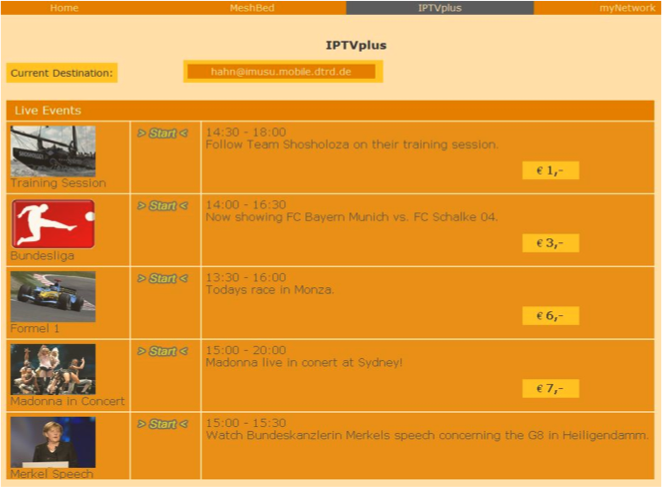
\includegraphics[width=\textwidth]{iptvplus}
  \caption{Old IPTVplus page}
  \label{fig:iptvplus}
\end{figure}

Basically, the user clicks on the button \textit{Start} to buy a content, then a popup appears to confirm the selection.
If confirmed, the user is \textit{charged} and the content starts playing in his default device.

From the user perspective this could be handled more elegantly, since the functionality is split between \idx{IPTVplus} and the \ida{PNAI}.
One of the goals of this work is integrating that functionality directly in the main \ida{PNAI} page.

This \idx{IPTVplus} application resides in a directory called \idc{scalenet} in the \idx{Apache} public folder.
The front page from where the user accesses all the \idx{ScaleNet} applications, and therefore also the \ida{PNAI}, is in that folder.
All these pages are written in \ida{PHP}.

Figure~\vref{fig:iptvdir} lists all the relevant \ida{PHP} files in this directory.
Some folders and files have been omitted because they are not relevant to this application.

\begin{figure}[htbp]
  \dirtree{%
    .1 scalenet/.
      .2 index.php.
      .2 sub/.
        .3 includes/.
          .4 auth.inc.php.
          .4 db.inc.php.
        .3 iptvplus/.
          .4 c2d.php.
          .4 inhalt.php.
          .4 popup.php.
        .3 IPTVplus.php.
        .3 mobile/.
        .3 mobile.php.
        .3 personal/.
          .4 sessions.php.
        .3 personal.php.
  }
  \caption{Old PHP directory}
  \label{fig:iptvdir}
\end{figure}

The front page is in \idc{index.php}, and it just contains several links to the sub-applications, that are in the \idc{sub} directory.
In the \idc{includes} directory there are two files used by almost every application: \idc{auth.inc.php} for authentication purposes and \idc{db.inc.php} for connecting to the \idx{HSS DB}.

The \idc{IPTVplus.php} page is the main page for the \idx{IPTVplus} application.
This page includes \idc{inhalt.php}, where most of the actual code is written.
In short, the output of this subpage is just a list of all available videos, ordered by categories, as seen in Figure~\vref{fig:iptvplus}.

Internally \idc{inhalt.php} gets the content in a very particular way.
Instead of querying the database directly, it connects to an additional socket at \url{webportal.imusu.mobile.dtrd.de:7001} to retrieve the list.
It does not matter which component really queries the database (the \ida{SSCON}) or how, because that was not changed during this work.

To that socket it sends the string \idc{list} followed by a carriage return (\texttt{\textbackslash{}r\textbackslash{}n}).
That command responds with the information of all content items, one by one.
For each content it sends in order the following information, separated by a carriage return: \idc{type}, \idc{content}, \idc{img}, \idc{text}, \idc{lov}, \idc{priority}, \idc{price}, \idc{description} and \idc{quality}.
The end of the transmission is marked by the raw string \idc{c2d}.

The very \ida{PHP} code is rather inefficient, because it actually asks for the content four times, one for each category.
That is, it opens the socket, send the command and receive the list four times.
Each time it discards all the videos from the other categories, instead of only asking one and then ordering the results before \emph{printing} the list.

As seen in Figure~\vref{fig:iptvplus}, the list shows the title for each content (\idc{text}), its icon, its description and its price.
A button with the text \emph{Start} allows the user to buy that content, by opening a popup to \idc{c2d.php} if the content is free or to \idc{popup.php} if it is not free.

\idc{c2d.php} receives four \idc{GET} parameters: the type of the stream, the desired quality, the id of the content and the impu of the destination device/user.
The link to this \ida{PHP} file looks like this:

\texttt{.../c2d.php?type=\emph{type}\&quality=\emph{quality}\&content=\emph{content}\&}

$\hookrightarrow$\texttt{impu=\emph{destimpu}}

This script sends a command to the \ida{SSCON} to start playing that content in that device.
It opens a socket exactly like in \idc{inhalt.php} and sends the string \idc{refer} followed by the parameters separated by spaces: the destination, the \ida{SIP} id of the \idx{Application Server}, the type, the content id and the quality.
The end of the command is marked by a carriage return.

\idc{popup.php} simply contains a confirmation page asking the user if he really wants to pay for that content, and redirects the user to the \idc{c2d.php} if he confirms it.
It receives two \idc{GET} parameters: the price and the link to the proper \idc{c2d.php} page (with the needed parameters already encoded in that \idx{URL}).
The link to this \ida{PHP} file looks like this:

\texttt{.../popup.php?price=\emph{price}\&link=\emph{linktoc2d}}

\idc{mobile.php} and the files contained in the \idc{mobile} folder have a mobile version of some of this applications.
This is a very limited version and it does not contain a \idx{PNAI} page, so this files where not even touched in this work.

\idc{personal.php} is the interface that controls some things related to the user.
In the \idc{personal} folder there are several subpages that can be embedded in \idc{personal.php} depending on a \idc{GET} parameter.
One of them is \idc{sessions.php}, simply a wrapper for the \idx{PNAI} page, and it consists of an iframe redirecting to the proper path in the \ida{OSGi} server.
Therefore the \idx{PNAI} page is integrated in this portal.

There are other pages available from the same portal, some of them refers to other services (like controlling/monitoring a Mesh network) but others are configuration pages for the user.
For example, in the \idc{personal} directory there are pages to control the buddy list (add/remove), control the device list (add/remove/edit), etc.
Since those pages were left untouched by this work, they are not explained.

% subsection iptvplus (end)

% section scalenet (end)